% Options for packages loaded elsewhere
\PassOptionsToPackage{unicode}{hyperref}
\PassOptionsToPackage{hyphens}{url}
%
\documentclass[
]{article}
\title{Class 10: Halloween Mini-Project}
\author{Andrew Kapinos}
\date{10/29/2021}

\usepackage{amsmath,amssymb}
\usepackage{lmodern}
\usepackage{iftex}
\ifPDFTeX
  \usepackage[T1]{fontenc}
  \usepackage[utf8]{inputenc}
  \usepackage{textcomp} % provide euro and other symbols
\else % if luatex or xetex
  \usepackage{unicode-math}
  \defaultfontfeatures{Scale=MatchLowercase}
  \defaultfontfeatures[\rmfamily]{Ligatures=TeX,Scale=1}
\fi
% Use upquote if available, for straight quotes in verbatim environments
\IfFileExists{upquote.sty}{\usepackage{upquote}}{}
\IfFileExists{microtype.sty}{% use microtype if available
  \usepackage[]{microtype}
  \UseMicrotypeSet[protrusion]{basicmath} % disable protrusion for tt fonts
}{}
\makeatletter
\@ifundefined{KOMAClassName}{% if non-KOMA class
  \IfFileExists{parskip.sty}{%
    \usepackage{parskip}
  }{% else
    \setlength{\parindent}{0pt}
    \setlength{\parskip}{6pt plus 2pt minus 1pt}}
}{% if KOMA class
  \KOMAoptions{parskip=half}}
\makeatother
\usepackage{xcolor}
\IfFileExists{xurl.sty}{\usepackage{xurl}}{} % add URL line breaks if available
\IfFileExists{bookmark.sty}{\usepackage{bookmark}}{\usepackage{hyperref}}
\hypersetup{
  pdftitle={Class 10: Halloween Mini-Project},
  pdfauthor={Andrew Kapinos},
  hidelinks,
  pdfcreator={LaTeX via pandoc}}
\urlstyle{same} % disable monospaced font for URLs
\usepackage[margin=1in]{geometry}
\usepackage{color}
\usepackage{fancyvrb}
\newcommand{\VerbBar}{|}
\newcommand{\VERB}{\Verb[commandchars=\\\{\}]}
\DefineVerbatimEnvironment{Highlighting}{Verbatim}{commandchars=\\\{\}}
% Add ',fontsize=\small' for more characters per line
\usepackage{framed}
\definecolor{shadecolor}{RGB}{248,248,248}
\newenvironment{Shaded}{\begin{snugshade}}{\end{snugshade}}
\newcommand{\AlertTok}[1]{\textcolor[rgb]{0.94,0.16,0.16}{#1}}
\newcommand{\AnnotationTok}[1]{\textcolor[rgb]{0.56,0.35,0.01}{\textbf{\textit{#1}}}}
\newcommand{\AttributeTok}[1]{\textcolor[rgb]{0.77,0.63,0.00}{#1}}
\newcommand{\BaseNTok}[1]{\textcolor[rgb]{0.00,0.00,0.81}{#1}}
\newcommand{\BuiltInTok}[1]{#1}
\newcommand{\CharTok}[1]{\textcolor[rgb]{0.31,0.60,0.02}{#1}}
\newcommand{\CommentTok}[1]{\textcolor[rgb]{0.56,0.35,0.01}{\textit{#1}}}
\newcommand{\CommentVarTok}[1]{\textcolor[rgb]{0.56,0.35,0.01}{\textbf{\textit{#1}}}}
\newcommand{\ConstantTok}[1]{\textcolor[rgb]{0.00,0.00,0.00}{#1}}
\newcommand{\ControlFlowTok}[1]{\textcolor[rgb]{0.13,0.29,0.53}{\textbf{#1}}}
\newcommand{\DataTypeTok}[1]{\textcolor[rgb]{0.13,0.29,0.53}{#1}}
\newcommand{\DecValTok}[1]{\textcolor[rgb]{0.00,0.00,0.81}{#1}}
\newcommand{\DocumentationTok}[1]{\textcolor[rgb]{0.56,0.35,0.01}{\textbf{\textit{#1}}}}
\newcommand{\ErrorTok}[1]{\textcolor[rgb]{0.64,0.00,0.00}{\textbf{#1}}}
\newcommand{\ExtensionTok}[1]{#1}
\newcommand{\FloatTok}[1]{\textcolor[rgb]{0.00,0.00,0.81}{#1}}
\newcommand{\FunctionTok}[1]{\textcolor[rgb]{0.00,0.00,0.00}{#1}}
\newcommand{\ImportTok}[1]{#1}
\newcommand{\InformationTok}[1]{\textcolor[rgb]{0.56,0.35,0.01}{\textbf{\textit{#1}}}}
\newcommand{\KeywordTok}[1]{\textcolor[rgb]{0.13,0.29,0.53}{\textbf{#1}}}
\newcommand{\NormalTok}[1]{#1}
\newcommand{\OperatorTok}[1]{\textcolor[rgb]{0.81,0.36,0.00}{\textbf{#1}}}
\newcommand{\OtherTok}[1]{\textcolor[rgb]{0.56,0.35,0.01}{#1}}
\newcommand{\PreprocessorTok}[1]{\textcolor[rgb]{0.56,0.35,0.01}{\textit{#1}}}
\newcommand{\RegionMarkerTok}[1]{#1}
\newcommand{\SpecialCharTok}[1]{\textcolor[rgb]{0.00,0.00,0.00}{#1}}
\newcommand{\SpecialStringTok}[1]{\textcolor[rgb]{0.31,0.60,0.02}{#1}}
\newcommand{\StringTok}[1]{\textcolor[rgb]{0.31,0.60,0.02}{#1}}
\newcommand{\VariableTok}[1]{\textcolor[rgb]{0.00,0.00,0.00}{#1}}
\newcommand{\VerbatimStringTok}[1]{\textcolor[rgb]{0.31,0.60,0.02}{#1}}
\newcommand{\WarningTok}[1]{\textcolor[rgb]{0.56,0.35,0.01}{\textbf{\textit{#1}}}}
\usepackage{longtable,booktabs,array}
\usepackage{calc} % for calculating minipage widths
% Correct order of tables after \paragraph or \subparagraph
\usepackage{etoolbox}
\makeatletter
\patchcmd\longtable{\par}{\if@noskipsec\mbox{}\fi\par}{}{}
\makeatother
% Allow footnotes in longtable head/foot
\IfFileExists{footnotehyper.sty}{\usepackage{footnotehyper}}{\usepackage{footnote}}
\makesavenoteenv{longtable}
\usepackage{graphicx}
\makeatletter
\def\maxwidth{\ifdim\Gin@nat@width>\linewidth\linewidth\else\Gin@nat@width\fi}
\def\maxheight{\ifdim\Gin@nat@height>\textheight\textheight\else\Gin@nat@height\fi}
\makeatother
% Scale images if necessary, so that they will not overflow the page
% margins by default, and it is still possible to overwrite the defaults
% using explicit options in \includegraphics[width, height, ...]{}
\setkeys{Gin}{width=\maxwidth,height=\maxheight,keepaspectratio}
% Set default figure placement to htbp
\makeatletter
\def\fps@figure{htbp}
\makeatother
\setlength{\emergencystretch}{3em} % prevent overfull lines
\providecommand{\tightlist}{%
  \setlength{\itemsep}{0pt}\setlength{\parskip}{0pt}}
\setcounter{secnumdepth}{-\maxdimen} % remove section numbering
\ifLuaTeX
  \usepackage{selnolig}  % disable illegal ligatures
\fi

\begin{document}
\maketitle

\hypertarget{importing-candy-data}{%
\subsection{1. Importing Candy Data}\label{importing-candy-data}}

First, let's import the dataset using read.csv(), then assign the data
to a data frame object using the first column as row titles.

\begin{Shaded}
\begin{Highlighting}[]
\NormalTok{url }\OtherTok{\textless{}{-}} \StringTok{"https://raw.githubusercontent.com/fivethirtyeight/data/master/candy{-}power{-}ranking/candy{-}data.csv"}
\NormalTok{candy\_file }\OtherTok{\textless{}{-}} \FunctionTok{read.csv}\NormalTok{(url)}
\NormalTok{candy }\OtherTok{=} \FunctionTok{data.frame}\NormalTok{(candy\_file, }\AttributeTok{row.names=}\DecValTok{1}\NormalTok{)}
\FunctionTok{rownames}\NormalTok{(candy) }\OtherTok{\textless{}{-}} \FunctionTok{gsub}\NormalTok{(}\StringTok{"Õ"}\NormalTok{,}\StringTok{"\textquotesingle{}"}\NormalTok{,}\FunctionTok{rownames}\NormalTok{(candy))}
\FunctionTok{head}\NormalTok{(candy)}
\end{Highlighting}
\end{Shaded}

\begin{verbatim}
##              chocolate fruity caramel peanutyalmondy nougat crispedricewafer
## 100 Grand            1      0       1              0      0                1
## 3 Musketeers         1      0       0              0      1                0
## One dime             0      0       0              0      0                0
## One quarter          0      0       0              0      0                0
## Air Heads            0      1       0              0      0                0
## Almond Joy           1      0       0              1      0                0
##              hard bar pluribus sugarpercent pricepercent winpercent
## 100 Grand       0   1        0        0.732        0.860   66.97173
## 3 Musketeers    0   1        0        0.604        0.511   67.60294
## One dime        0   0        0        0.011        0.116   32.26109
## One quarter     0   0        0        0.011        0.511   46.11650
## Air Heads       0   0        0        0.906        0.511   52.34146
## Almond Joy      0   1        0        0.465        0.767   50.34755
\end{verbatim}

\begin{quote}
Q1. How many different candy types are in this dataset?
\end{quote}

\begin{Shaded}
\begin{Highlighting}[]
\FunctionTok{nrow}\NormalTok{(candy)}
\end{Highlighting}
\end{Shaded}

\begin{verbatim}
## [1] 85
\end{verbatim}

There are 85 types of candy in the dataset.

\begin{quote}
Q2. How many fruity candy types are in the dataset?
\end{quote}

\begin{Shaded}
\begin{Highlighting}[]
\FunctionTok{sum}\NormalTok{(candy}\SpecialCharTok{$}\NormalTok{fruity)}
\end{Highlighting}
\end{Shaded}

\begin{verbatim}
## [1] 38
\end{verbatim}

There are 38 fruity candy types.

\hypertarget{what-is-your-favorite-candy}{%
\subsection{2. What is your favorite
candy?}\label{what-is-your-favorite-candy}}

The variable ``winpercent'' is the percentage of people who prefer this
candy over another randlomly chosen candy in the dataset.

Let's determine the winpercent value for Twix:

\begin{Shaded}
\begin{Highlighting}[]
\NormalTok{candy[}\StringTok{"Twix"}\NormalTok{,]}\SpecialCharTok{$}\NormalTok{winpercent}
\end{Highlighting}
\end{Shaded}

\begin{verbatim}
## [1] 81.64291
\end{verbatim}

\begin{quote}
Q3. What is your favorite candy in the dataset and what is it's
winpercent value?
\end{quote}

Reese's Peanut Butter cup

\begin{Shaded}
\begin{Highlighting}[]
\NormalTok{candy[}\StringTok{"Reese\textquotesingle{}s Peanut Butter cup"}\NormalTok{,]}\SpecialCharTok{$}\NormalTok{winpercent}
\end{Highlighting}
\end{Shaded}

\begin{verbatim}
## [1] 84.18029
\end{verbatim}

\begin{quote}
Q4. What is the winpercent value for ``Kit Kat''?
\end{quote}

\begin{Shaded}
\begin{Highlighting}[]
\NormalTok{candy[}\StringTok{"Kit Kat"}\NormalTok{,]}\SpecialCharTok{$}\NormalTok{winpercent}
\end{Highlighting}
\end{Shaded}

\begin{verbatim}
## [1] 76.7686
\end{verbatim}

\begin{quote}
Q5. What is the winpercent value for ``Tootsie Roll Snack Bars''?
\end{quote}

\begin{Shaded}
\begin{Highlighting}[]
\NormalTok{candy[}\StringTok{"Tootsie Roll Snack Bars"}\NormalTok{,]}\SpecialCharTok{$}\NormalTok{winpercent}
\end{Highlighting}
\end{Shaded}

\begin{verbatim}
## [1] 49.6535
\end{verbatim}

Let's use skim() in the skimr package to get a quickl overview of the
dataset.

\begin{Shaded}
\begin{Highlighting}[]
\FunctionTok{library}\NormalTok{(}\StringTok{"skimr"}\NormalTok{)}
\FunctionTok{skim}\NormalTok{(candy)}
\end{Highlighting}
\end{Shaded}

\begin{longtable}[]{@{}ll@{}}
\caption{Data summary}\tabularnewline
\toprule
\endhead
Name & candy \\
Number of rows & 85 \\
Number of columns & 12 \\
\_\_\_\_\_\_\_\_\_\_\_\_\_\_\_\_\_\_\_\_\_\_\_ & \\
Column type frequency: & \\
numeric & 12 \\
\_\_\_\_\_\_\_\_\_\_\_\_\_\_\_\_\_\_\_\_\_\_\_\_ & \\
Group variables & None \\
\bottomrule
\end{longtable}

\textbf{Variable type: numeric}

\begin{longtable}[]{@{}lrrrrrrrrrl@{}}
\toprule
skim\_variable & n\_missing & complete\_rate & mean & sd & p0 & p25 &
p50 & p75 & p100 & hist \\
\midrule
\endhead
chocolate & 0 & 1 & 0.44 & 0.50 & 0.00 & 0.00 & 0.00 & 1.00 & 1.00 &
▇▁▁▁▆ \\
fruity & 0 & 1 & 0.45 & 0.50 & 0.00 & 0.00 & 0.00 & 1.00 & 1.00 &
▇▁▁▁▆ \\
caramel & 0 & 1 & 0.16 & 0.37 & 0.00 & 0.00 & 0.00 & 0.00 & 1.00 &
▇▁▁▁▂ \\
peanutyalmondy & 0 & 1 & 0.16 & 0.37 & 0.00 & 0.00 & 0.00 & 0.00 & 1.00
& ▇▁▁▁▂ \\
nougat & 0 & 1 & 0.08 & 0.28 & 0.00 & 0.00 & 0.00 & 0.00 & 1.00 &
▇▁▁▁▁ \\
crispedricewafer & 0 & 1 & 0.08 & 0.28 & 0.00 & 0.00 & 0.00 & 0.00 &
1.00 & ▇▁▁▁▁ \\
hard & 0 & 1 & 0.18 & 0.38 & 0.00 & 0.00 & 0.00 & 0.00 & 1.00 & ▇▁▁▁▂ \\
bar & 0 & 1 & 0.25 & 0.43 & 0.00 & 0.00 & 0.00 & 0.00 & 1.00 & ▇▁▁▁▂ \\
pluribus & 0 & 1 & 0.52 & 0.50 & 0.00 & 0.00 & 1.00 & 1.00 & 1.00 &
▇▁▁▁▇ \\
sugarpercent & 0 & 1 & 0.48 & 0.28 & 0.01 & 0.22 & 0.47 & 0.73 & 0.99 &
▇▇▇▇▆ \\
pricepercent & 0 & 1 & 0.47 & 0.29 & 0.01 & 0.26 & 0.47 & 0.65 & 0.98 &
▇▇▇▇▆ \\
winpercent & 0 & 1 & 50.32 & 14.71 & 22.45 & 39.14 & 47.83 & 59.86 &
84.18 & ▃▇▆▅▂ \\
\bottomrule
\end{longtable}

\begin{quote}
Q6. Is there any variable/column that looks to be on a different scale
to the majority of the other columns in the dataset?
\end{quote}

Yes; the last variable is scaled differently (0-100 instead of 0-1, as
the other variables are scaled).

\begin{quote}
Q7. What do you think a zero and one represent for the candy\$chocolate
column?
\end{quote}

Zero means that the candy type is not chocolatey, while a one means that
it is.

\begin{quote}
Q8. Plot a histogram of winpercent values
\end{quote}

\begin{Shaded}
\begin{Highlighting}[]
\FunctionTok{hist}\NormalTok{(candy}\SpecialCharTok{$}\NormalTok{winpercent)}
\end{Highlighting}
\end{Shaded}

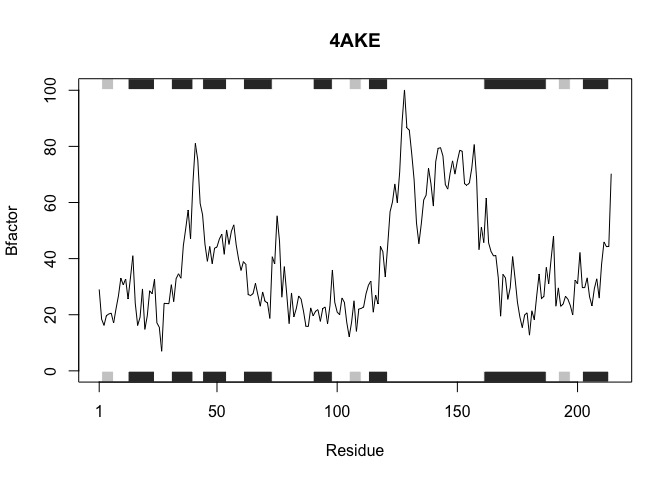
\includegraphics{class10_files/figure-latex/unnamed-chunk-9-1.pdf}

\begin{quote}
Q9. Is the distribution of winpercent values symmetrical?
\end{quote}

No, the distribution skews right (positive skew).

\begin{quote}
Q10. Is the center of the distribution above or below 50\%?
\end{quote}

Below 50\%.

\begin{quote}
Q11. On average is chocolate candy higher or lower ranked than fruit
candy?
\end{quote}

\begin{Shaded}
\begin{Highlighting}[]
\FunctionTok{t.test}\NormalTok{(candy}\SpecialCharTok{$}\NormalTok{winpercent[}\FunctionTok{as.logical}\NormalTok{(candy}\SpecialCharTok{$}\NormalTok{chocolate)],candy}\SpecialCharTok{$}\NormalTok{winpercent[}\FunctionTok{as.logical}\NormalTok{(candy}\SpecialCharTok{$}\NormalTok{fruit)])}
\end{Highlighting}
\end{Shaded}

\begin{verbatim}
## 
##  Welch Two Sample t-test
## 
## data:  candy$winpercent[as.logical(candy$chocolate)] and candy$winpercent[as.logical(candy$fruit)]
## t = 6.2582, df = 68.882, p-value = 2.871e-08
## alternative hypothesis: true difference in means is not equal to 0
## 95 percent confidence interval:
##  11.44563 22.15795
## sample estimates:
## mean of x mean of y 
##  60.92153  44.11974
\end{verbatim}

On average, chocolate has a higher win percent than fruit. The mean
winpercent for chocolate = 60.92153, while the mean winpercent for fruit
= 44.11974.

\begin{quote}
Q12. Is this difference statistically significant?
\end{quote}

Yes, it is significant using a significance threshold of p\textless0.05.
The p-value for this comparison is 2.871e-08.

\hypertarget{overall-candy-rankings}{%
\subsection{3. Overall candy rankings}\label{overall-candy-rankings}}

Let's order the dataset based on the winpercent variable, in ascending
order, using dplyr and arrange().

\begin{quote}
Q13. What are the five least liked candy types in this set?
\end{quote}

\begin{Shaded}
\begin{Highlighting}[]
\FunctionTok{library}\NormalTok{(}\StringTok{"dplyr"}\NormalTok{)}
\end{Highlighting}
\end{Shaded}

\begin{verbatim}
## 
## Attaching package: 'dplyr'
\end{verbatim}

\begin{verbatim}
## The following objects are masked from 'package:stats':
## 
##     filter, lag
\end{verbatim}

\begin{verbatim}
## The following objects are masked from 'package:base':
## 
##     intersect, setdiff, setequal, union
\end{verbatim}

\begin{Shaded}
\begin{Highlighting}[]
\NormalTok{candy }\SpecialCharTok{\%\textgreater{}\%} \FunctionTok{arrange}\NormalTok{(winpercent) }\SpecialCharTok{\%\textgreater{}\%} \FunctionTok{head}\NormalTok{(}\DecValTok{5}\NormalTok{)}
\end{Highlighting}
\end{Shaded}

\begin{verbatim}
##                    chocolate fruity caramel peanutyalmondy nougat
## Nik L Nip                  0      1       0              0      0
## Boston Baked Beans         0      0       0              1      0
## Chiclets                   0      1       0              0      0
## Super Bubble               0      1       0              0      0
## Jawbusters                 0      1       0              0      0
##                    crispedricewafer hard bar pluribus sugarpercent pricepercent
## Nik L Nip                         0    0   0        1        0.197        0.976
## Boston Baked Beans                0    0   0        1        0.313        0.511
## Chiclets                          0    0   0        1        0.046        0.325
## Super Bubble                      0    0   0        0        0.162        0.116
## Jawbusters                        0    1   0        1        0.093        0.511
##                    winpercent
## Nik L Nip            22.44534
## Boston Baked Beans   23.41782
## Chiclets             24.52499
## Super Bubble         27.30386
## Jawbusters           28.12744
\end{verbatim}

The five least liked candies are Nik L Nip, Boston Baked Beans,
Chiclets, Super Bubble, and Jawbusters.

\begin{quote}
Q14. What are the top 5 all time favorite candy types out of this set?
\end{quote}

\begin{Shaded}
\begin{Highlighting}[]
\NormalTok{candy }\SpecialCharTok{\%\textgreater{}\%} \FunctionTok{arrange}\NormalTok{(}\FunctionTok{desc}\NormalTok{(winpercent)) }\SpecialCharTok{\%\textgreater{}\%} \FunctionTok{head}\NormalTok{(}\DecValTok{5}\NormalTok{)}
\end{Highlighting}
\end{Shaded}

\begin{verbatim}
##                           chocolate fruity caramel peanutyalmondy nougat
## Reese's Peanut Butter cup         1      0       0              1      0
## Reese's Miniatures                1      0       0              1      0
## Twix                              1      0       1              0      0
## Kit Kat                           1      0       0              0      0
## Snickers                          1      0       1              1      1
##                           crispedricewafer hard bar pluribus sugarpercent
## Reese's Peanut Butter cup                0    0   0        0        0.720
## Reese's Miniatures                       0    0   0        0        0.034
## Twix                                     1    0   1        0        0.546
## Kit Kat                                  1    0   1        0        0.313
## Snickers                                 0    0   1        0        0.546
##                           pricepercent winpercent
## Reese's Peanut Butter cup        0.651   84.18029
## Reese's Miniatures               0.279   81.86626
## Twix                             0.906   81.64291
## Kit Kat                          0.511   76.76860
## Snickers                         0.651   76.67378
\end{verbatim}

The top 5 all time favorite candy types are Reese's Peanut Butter cup,
Reese's Miniatures, Twix, Kit Kat, and Snickers.

\begin{quote}
Q15. Make a first barplot of candy ranking based on winpercent values.
\end{quote}

\begin{Shaded}
\begin{Highlighting}[]
\FunctionTok{library}\NormalTok{(ggplot2)}
\FunctionTok{ggplot}\NormalTok{(candy) }\SpecialCharTok{+}
  \FunctionTok{aes}\NormalTok{(winpercent, }\FunctionTok{rownames}\NormalTok{(candy)) }\SpecialCharTok{+}
  \FunctionTok{geom\_col}\NormalTok{()}
\end{Highlighting}
\end{Shaded}

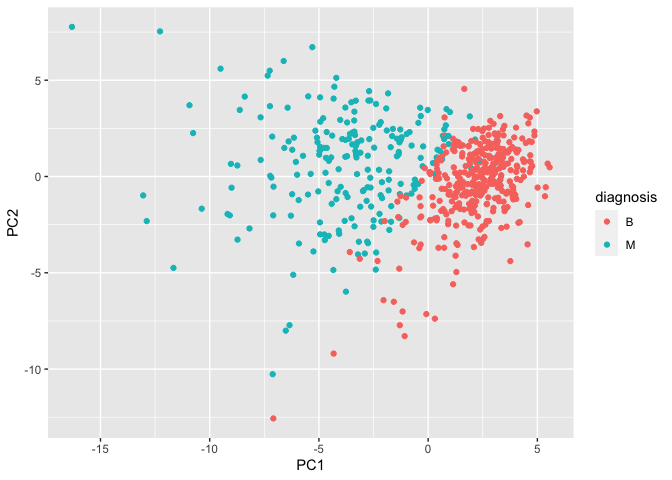
\includegraphics{class10_files/figure-latex/unnamed-chunk-13-1.pdf}

\begin{quote}
Q16. This is quite ugly, use the reorder() function to get the bars
sorted by winpercent?
\end{quote}

\begin{Shaded}
\begin{Highlighting}[]
\FunctionTok{ggplot}\NormalTok{(candy) }\SpecialCharTok{+}
  \FunctionTok{aes}\NormalTok{(winpercent, }\FunctionTok{reorder}\NormalTok{(}\FunctionTok{rownames}\NormalTok{(candy),winpercent)) }\SpecialCharTok{+}
  \FunctionTok{geom\_col}\NormalTok{() }\SpecialCharTok{+} \FunctionTok{labs}\NormalTok{(}\AttributeTok{x=}\StringTok{"Win percent"}\NormalTok{,}\AttributeTok{y=}\StringTok{"Candy type"}\NormalTok{)}
\end{Highlighting}
\end{Shaded}

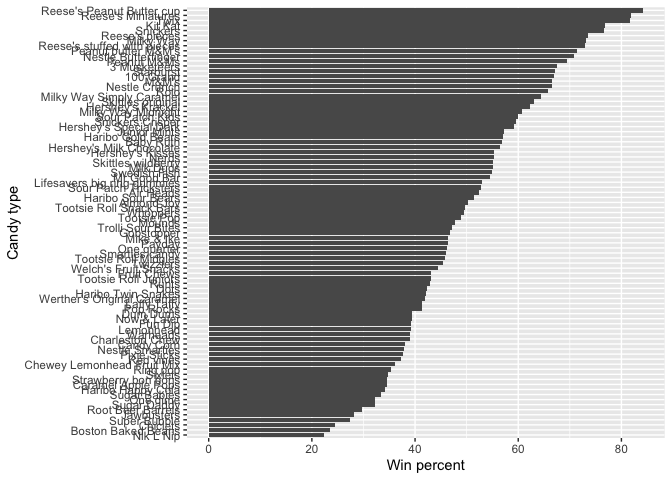
\includegraphics{class10_files/figure-latex/unnamed-chunk-14-1.pdf}

\begin{Shaded}
\begin{Highlighting}[]
\NormalTok{my\_cols}\OtherTok{=}\FunctionTok{rep}\NormalTok{(}\StringTok{"black"}\NormalTok{, }\FunctionTok{nrow}\NormalTok{(candy))}
\NormalTok{my\_cols[}\FunctionTok{as.logical}\NormalTok{(candy}\SpecialCharTok{$}\NormalTok{chocolate)] }\OtherTok{=} \StringTok{"chocolate"}
\NormalTok{my\_cols[}\FunctionTok{as.logical}\NormalTok{(candy}\SpecialCharTok{$}\NormalTok{bar)] }\OtherTok{=} \StringTok{"brown"}
\NormalTok{my\_cols[}\FunctionTok{as.logical}\NormalTok{(candy}\SpecialCharTok{$}\NormalTok{fruity)] }\OtherTok{=} \StringTok{"pink"}
\FunctionTok{ggplot}\NormalTok{(candy) }\SpecialCharTok{+}
  \FunctionTok{aes}\NormalTok{(winpercent, }\FunctionTok{reorder}\NormalTok{(}\FunctionTok{rownames}\NormalTok{(candy),winpercent)) }\SpecialCharTok{+}
  \FunctionTok{geom\_col}\NormalTok{(}\AttributeTok{fill=}\NormalTok{my\_cols) }\SpecialCharTok{+} \FunctionTok{labs}\NormalTok{(}\AttributeTok{x=}\StringTok{"Win percent"}\NormalTok{,}\AttributeTok{y=}\StringTok{"Candy type"}\NormalTok{)}
\end{Highlighting}
\end{Shaded}

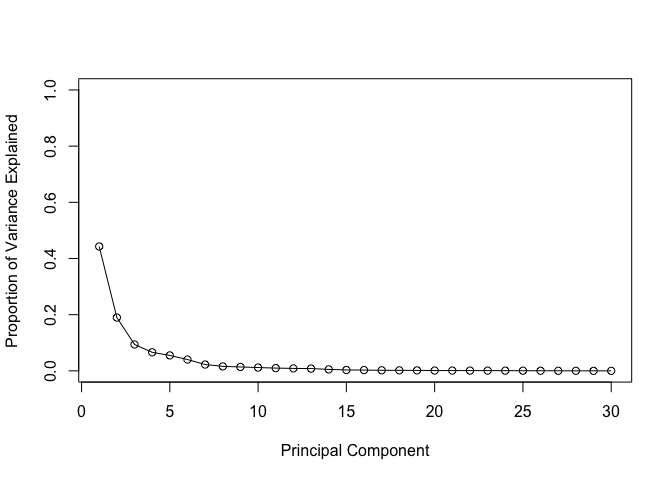
\includegraphics{class10_files/figure-latex/unnamed-chunk-15-1.pdf}

\begin{quote}
Q17. What is the worst ranked chocolate candy?
\end{quote}

Sixlets is the worst ranked chocolate candy.

\begin{quote}
Q18. What is the best ranked fruity candy?
\end{quote}

Starburst is the best ranked fruity candy.

\hypertarget{taking-a-look-at-pricepercent}{%
\subsection{4. Taking a look at
pricepercent}\label{taking-a-look-at-pricepercent}}

\begin{Shaded}
\begin{Highlighting}[]
\FunctionTok{library}\NormalTok{(ggrepel)}

\CommentTok{\# How about a plot of price vs win}
\FunctionTok{ggplot}\NormalTok{(candy) }\SpecialCharTok{+}
  \FunctionTok{aes}\NormalTok{(winpercent, pricepercent, }\AttributeTok{label=}\FunctionTok{rownames}\NormalTok{(candy)) }\SpecialCharTok{+}
  \FunctionTok{geom\_point}\NormalTok{(}\AttributeTok{col=}\NormalTok{my\_cols) }\SpecialCharTok{+} 
  \FunctionTok{geom\_text\_repel}\NormalTok{(}\AttributeTok{col=}\NormalTok{my\_cols, }\AttributeTok{size=}\FloatTok{1.5}\NormalTok{, }\AttributeTok{max.overlaps =} \DecValTok{7}\NormalTok{)}
\end{Highlighting}
\end{Shaded}

\begin{verbatim}
## Warning: ggrepel: 5 unlabeled data points (too many overlaps). Consider
## increasing max.overlaps
\end{verbatim}

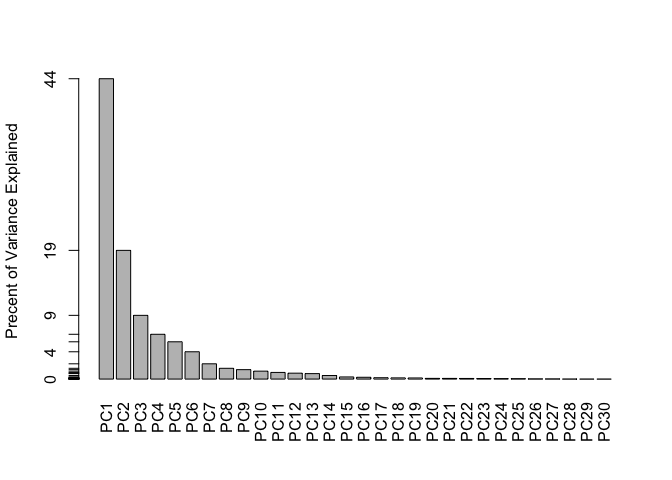
\includegraphics{class10_files/figure-latex/unnamed-chunk-16-1.pdf}

\begin{quote}
Q19. Which candy type is the highest ranked in terms of winpercent for
the least money - i.e.~offers the most bang for your buck?
\end{quote}

Reese's Miniatures is the highest ranked in terms of winpercent for the
least money.

\begin{quote}
Q20. What are the top 5 most expensive candy types in the dataset and of
these which is the least popular?
\end{quote}

\begin{Shaded}
\begin{Highlighting}[]
\NormalTok{candy }\SpecialCharTok{\%\textgreater{}\%} \FunctionTok{arrange}\NormalTok{(}\FunctionTok{desc}\NormalTok{(pricepercent)) }\SpecialCharTok{\%\textgreater{}\%} \FunctionTok{head}\NormalTok{(}\DecValTok{5}\NormalTok{)}
\end{Highlighting}
\end{Shaded}

\begin{verbatim}
##                          chocolate fruity caramel peanutyalmondy nougat
## Nik L Nip                        0      1       0              0      0
## Nestle Smarties                  1      0       0              0      0
## Ring pop                         0      1       0              0      0
## Hershey's Krackel                1      0       0              0      0
## Hershey's Milk Chocolate         1      0       0              0      0
##                          crispedricewafer hard bar pluribus sugarpercent
## Nik L Nip                               0    0   0        1        0.197
## Nestle Smarties                         0    0   0        1        0.267
## Ring pop                                0    1   0        0        0.732
## Hershey's Krackel                       1    0   1        0        0.430
## Hershey's Milk Chocolate                0    0   1        0        0.430
##                          pricepercent winpercent
## Nik L Nip                       0.976   22.44534
## Nestle Smarties                 0.976   37.88719
## Ring pop                        0.965   35.29076
## Hershey's Krackel               0.918   62.28448
## Hershey's Milk Chocolate        0.918   56.49050
\end{verbatim}

Nik L Nip, Nestle Smarties, Ring pop, Hershey's Krackel, and Hershey's
Milk Chocolate are the 5 most expensive candy types. Of these, the least
popular is Nik L Nip.

\begin{quote}
Optional Q21. Make a barplot again with geom\_col() this time using
pricepercent and then improve this step by step, first ordering the
x-axis by value and finally making a so called ``dot chat'' or
``lollipop'' chart by swapping geom\_col() for geom\_point() +
geom\_segment().
\end{quote}

\begin{Shaded}
\begin{Highlighting}[]
\FunctionTok{ggplot}\NormalTok{(candy) }\SpecialCharTok{+}
  \FunctionTok{aes}\NormalTok{(pricepercent, }\FunctionTok{reorder}\NormalTok{(}\FunctionTok{rownames}\NormalTok{(candy),pricepercent)) }\SpecialCharTok{+}
  \FunctionTok{geom\_col}\NormalTok{() }\SpecialCharTok{+} \FunctionTok{labs}\NormalTok{(}\AttributeTok{x=}\StringTok{"Price percent"}\NormalTok{,}\AttributeTok{y=}\StringTok{"Candy type"}\NormalTok{)}
\end{Highlighting}
\end{Shaded}

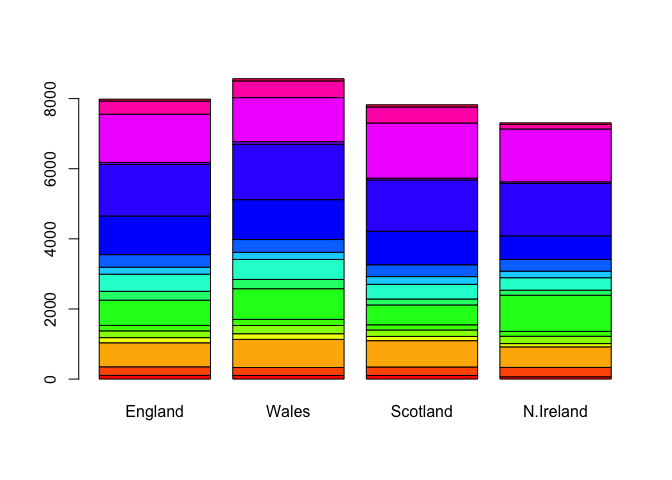
\includegraphics{class10_files/figure-latex/unnamed-chunk-18-1.pdf}

\begin{Shaded}
\begin{Highlighting}[]
\FunctionTok{ggplot}\NormalTok{(candy) }\SpecialCharTok{+}
  \FunctionTok{aes}\NormalTok{(pricepercent, }\FunctionTok{reorder}\NormalTok{(}\FunctionTok{rownames}\NormalTok{(candy), pricepercent)) }\SpecialCharTok{+}
  \FunctionTok{geom\_segment}\NormalTok{(}\FunctionTok{aes}\NormalTok{(}\AttributeTok{yend =} \FunctionTok{reorder}\NormalTok{(}\FunctionTok{rownames}\NormalTok{(candy), pricepercent), }\AttributeTok{xend =} \DecValTok{0}\NormalTok{), }\AttributeTok{col=}\StringTok{"gray40"}\NormalTok{) }\SpecialCharTok{+}
    \FunctionTok{geom\_point}\NormalTok{() }\SpecialCharTok{+} \FunctionTok{labs}\NormalTok{(}\AttributeTok{x=}\StringTok{"Price percent"}\NormalTok{,}\AttributeTok{y=}\StringTok{"Candy type"}\NormalTok{)}
\end{Highlighting}
\end{Shaded}

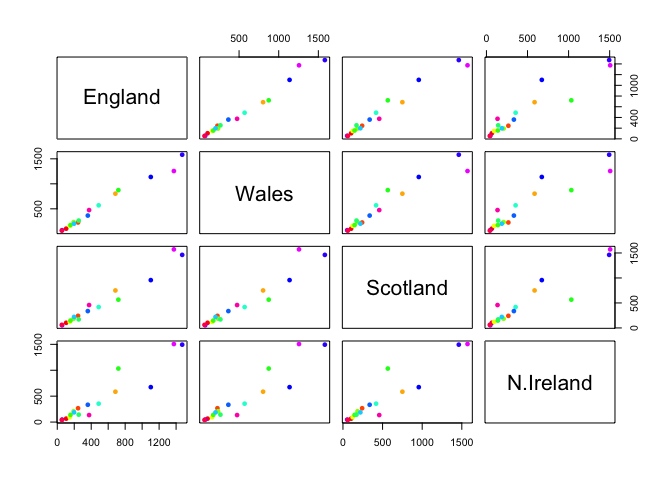
\includegraphics{class10_files/figure-latex/unnamed-chunk-19-1.pdf}

\hypertarget{exploring-the-correlation-structure}{%
\subsection{Exploring the correlation
structure}\label{exploring-the-correlation-structure}}

Now that we've explored the dataset a little, let's see how the
variables interact with one another, using the corrplot package to get a
correlation matrix.

\begin{Shaded}
\begin{Highlighting}[]
\FunctionTok{library}\NormalTok{(corrplot)}
\end{Highlighting}
\end{Shaded}

\begin{verbatim}
## corrplot 0.90 loaded
\end{verbatim}

\begin{Shaded}
\begin{Highlighting}[]
\NormalTok{cij }\OtherTok{\textless{}{-}} \FunctionTok{cor}\NormalTok{(candy)}
\FunctionTok{corrplot}\NormalTok{(cij)}
\end{Highlighting}
\end{Shaded}

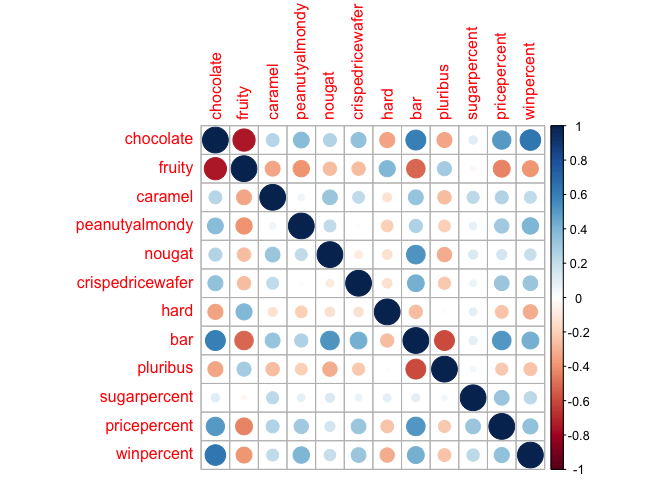
\includegraphics{class10_files/figure-latex/unnamed-chunk-20-1.pdf}

\begin{quote}
Q22. Examining this plot, what two variables are anti-correlated
(i.e.~have minus values)?
\end{quote}

\begin{enumerate}
\def\labelenumi{(\arabic{enumi})}
\tightlist
\item
  Chocolate and fruity, (2) Bar and pluribus, (3) fruity and bar
\end{enumerate}

\begin{quote}
Q23. Similarly, what two variables are most positively correlated?
\end{quote}

\begin{enumerate}
\def\labelenumi{(\arabic{enumi})}
\tightlist
\item
  Chocolate and winpercent, (2) Chocolate and bar, (3) Chocolate and
  pricepercent
\end{enumerate}

\hypertarget{principal-component-analysis}{%
\subsection{6. Principal Component
Analysis}\label{principal-component-analysis}}

Let's perform PCA on our candy dataset, using the prcomp() function and
the scale=TRUE argument.

\begin{Shaded}
\begin{Highlighting}[]
\NormalTok{pca }\OtherTok{\textless{}{-}} \FunctionTok{prcomp}\NormalTok{(candy,}\AttributeTok{scale=}\ConstantTok{TRUE}\NormalTok{)}
\FunctionTok{summary}\NormalTok{(pca)}
\end{Highlighting}
\end{Shaded}

\begin{verbatim}
## Importance of components:
##                           PC1    PC2    PC3     PC4    PC5     PC6     PC7
## Standard deviation     2.0788 1.1378 1.1092 1.07533 0.9518 0.81923 0.81530
## Proportion of Variance 0.3601 0.1079 0.1025 0.09636 0.0755 0.05593 0.05539
## Cumulative Proportion  0.3601 0.4680 0.5705 0.66688 0.7424 0.79830 0.85369
##                            PC8     PC9    PC10    PC11    PC12
## Standard deviation     0.74530 0.67824 0.62349 0.43974 0.39760
## Proportion of Variance 0.04629 0.03833 0.03239 0.01611 0.01317
## Cumulative Proportion  0.89998 0.93832 0.97071 0.98683 1.00000
\end{verbatim}

Let's plot our PCA score plot of PC1 v. PC2.

\begin{Shaded}
\begin{Highlighting}[]
\FunctionTok{plot}\NormalTok{(pca}\SpecialCharTok{$}\NormalTok{x[,}\DecValTok{1}\SpecialCharTok{:}\DecValTok{2}\NormalTok{])}
\end{Highlighting}
\end{Shaded}

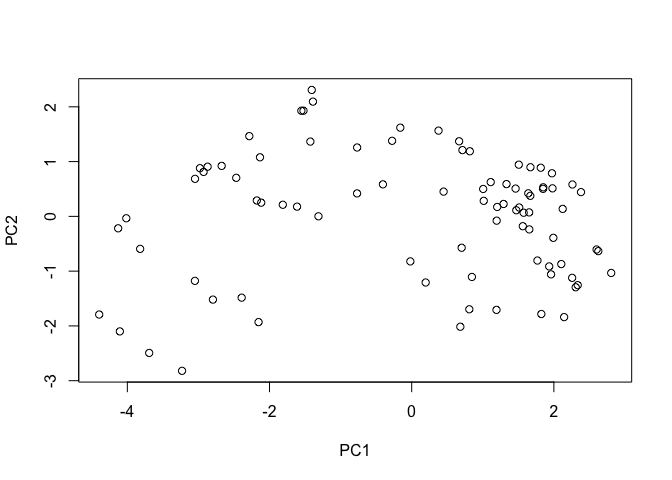
\includegraphics{class10_files/figure-latex/unnamed-chunk-22-1.pdf}

Let's change the plotting character and add some color.

\begin{Shaded}
\begin{Highlighting}[]
\FunctionTok{plot}\NormalTok{(pca}\SpecialCharTok{$}\NormalTok{x[,}\DecValTok{1}\SpecialCharTok{:}\DecValTok{2}\NormalTok{], }\AttributeTok{col=}\NormalTok{my\_cols, }\AttributeTok{pch=}\DecValTok{16}\NormalTok{)}
\end{Highlighting}
\end{Shaded}

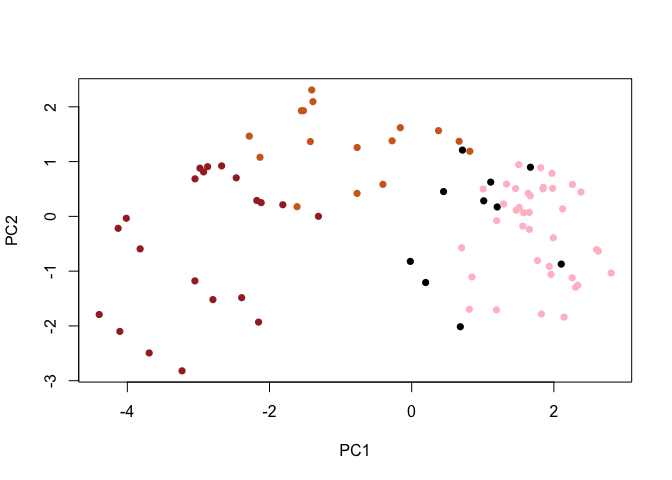
\includegraphics{class10_files/figure-latex/unnamed-chunk-23-1.pdf}

\end{document}
